\documentclass{beamer}

\usepackage[francais]{babel}
\usepackage[T1]{fontenc}
\usepackage[utf8]{inputenc}
\usepackage{beamerthemecs}
\usepackage{beamerouterthemecs}
\usepackage{beamerfontthemecs}
\usepackage{beamerinnerthemecs}
\usepackage{beamercolorthemecs}

\usetheme{cs}
\useoutertheme{cs}
\usefonttheme{cs}
\useinnertheme{cs}
\usecolortheme{cs}

\title[Visualisation de traces réseaux]{Visualisation de traces réseaux}
\author{\textbf{Thibault \textsc{Lengagne}et Nicolas \textsc{Ngô-Maï}}}
\institute{Centrale Supélec - Campus de Rennes}

\begin{document}

  \begin{frame}
    \titlepage
  \end{frame}
  
  \AtBeginSection[] {
    \begin{frame}
      \frametitle{Plan}
      \tableofcontents[currentsection, hideothersubsections, pausesubsections]
    \end{frame} 
  }

 \section{Retour sur les choix technologiques}
  \begin{frame}
    \frametitle{Rappel du Sujet}
    \begin{itemize}
     \item Le but est de créer un outil destiné aux pentesters, permettant d'analyser efficacement une trace réseau.
     \item L'attaquant dispose d'une trace réseau mais n'a aucune connaissance de ce réseau.
     \item Un fichier pcap devient rapidement très volumineux et son analyse est laborieuse, nécessitant l'utilisation de plusieurs outils.
    \end{itemize}
  \end{frame}
  
  \begin{frame}
    \frametitle{Rappel du Sujet}
    L'attaquant espère soutirer des informations sur le réseau :
    \begin{itemize}
      \item Les adresse IP identifiées ( + géolocalisation, résolution DNS)
      \item Les protocoles utilisés ( en particulier non chiffrés ou mal configurés)
      \item Les noeuds importants du réseau (serveur de fichier, DNS, LDAP...)
      \item Extraire des traces réseaux filtrées, extraire les données sensibles
    \end{itemize}
  \end{frame}

  \begin{frame}
   \frametitle{Retour sur les choix technologiques}
    \begin{itemize}
      \item Nous voulions à l'origine interfacer plusieurs outils (Ettercap, ChaosReader, tcptrace...) 
      \item Finalement, Scapy nous permet de manipuler la trace réseau de façon satisfaisante.
      \item Enfin, le choix initial de PyQt a été remplacé par une interface web.
    \end{itemize}
  \end{frame}
  
  \begin{frame}
  \frametitle{Retour sur les objectifs fixés}
    Nous avons d'ores et déjà remplis les objectifs suivants :
    \begin{itemize}
     \item Extraction de sessions, des utilisateurs, et des protocoles
     \item Création de statistiques, extraction des données en clair
     \item Visualisation en barre parallèle
    \end{itemize}
  \end{frame}
  
  \section{Détails techniques}
  \begin{frame}
  \frametitle{Nos choix de technologies}
   \begin{itemize}
    \item Le travail s'articule principalement autour de deux technologies :
    Scapy et D3.js
    \item Scapy est une librairie Python pour faire de la manipulation de trames
    réseaux
    \item D3.js est une librairie Javascript qui permet de faire de la
    manipulation de SVG lié à des données.
   \end{itemize}
  \end{frame}
  
  \begin{frame}
  \frametitle{Nos choix de technologies}
   \begin{itemize}
    \item Serveur web Flask (Python) associé à une base de données Postgres et
    un ORM python, SQLAlchemy
    \item Pour réaliser un update continu en fonction des données analysées par
    le serveur, nous avons installé SocketIO
   \end{itemize}
  \end{frame}
  
  \begin{frame}
  \frametitle{Présentation de D3.js}
   \begin{itemize}
    \item Framework JS pour faire de la manipulation d'objets du DOM en les
    liant à des données
    \item On peut ainsi faire apparaître des balises html ou SVG en fonction
    d'une donnée arbitraire
    \item Du coup, les graphes s'adaptent aux données de façon automatique
    \\-\textgreater \hspace{0.3mm} La structure des données est ce qui détermine
    le graphe
   \end{itemize}
  \end{frame}
  
  \begin{frame}
  \frametitle{Démonstation D3.js}
  % Ici démonstration live de 3min
  \end{frame}

  \begin{frame}
   Quatres tables dans la base de données :
   \begin{center}
    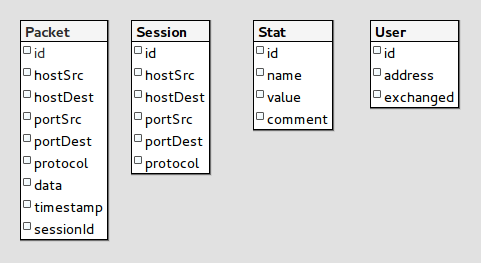
\includegraphics[scale=0.6]{postgre.png}
   \end{center}
  \end{frame}
  
  \begin{frame}
    \frametitle{Analyse du fichier pcap}
    \begin{itemize}
     \item La libraire Scapy permet de lire nos fichiers, puis de manipuler les packets.
     \item Une fonction parcourt tous les paquets. Les tables User et Stats sont alimentées 
     \item Une fonction parcourt tous les sessions. Les tables Session et Trames sont alimentées
    \end{itemize}
    %Montrer le code réduit
  \end{frame}
  
  \begin{frame}
    \frametitle{Performances du parser}
    \begin{itemize}
     \item Les fichiers pcap peuvent atteindre plusieurs Giga assez rapidement. 
     \item L'écriture dans la base de donnée étant couteuse,le programme écrit dans la base de donnée une seule fois, à la fin de la collecte des données
     \item Nous réalisons nos tests sur des traces d'entreprise anonymisées
     (ftp://ftp.bro-ids.org/enterprise-traces/hdr-traces05/)
    \end{itemize}
    %Afficher les résultats
  \end{frame}
  
  \begin{frame}
    \begin{center}
      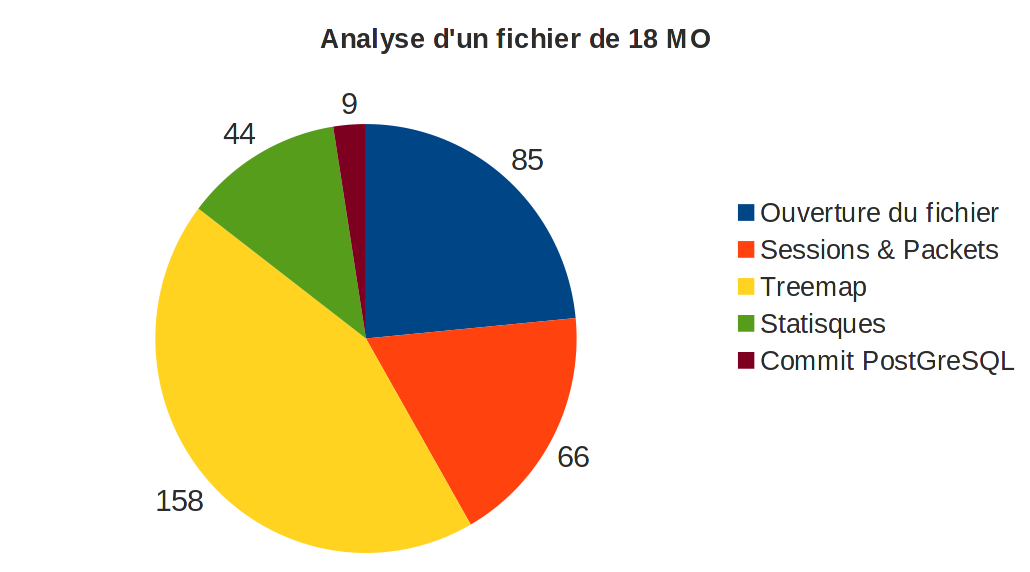
\includegraphics[scale=0.3]{parse-time.png}
    \end{center} 
  \end{frame}
  
  \begin{frame}
    \begin{center}
       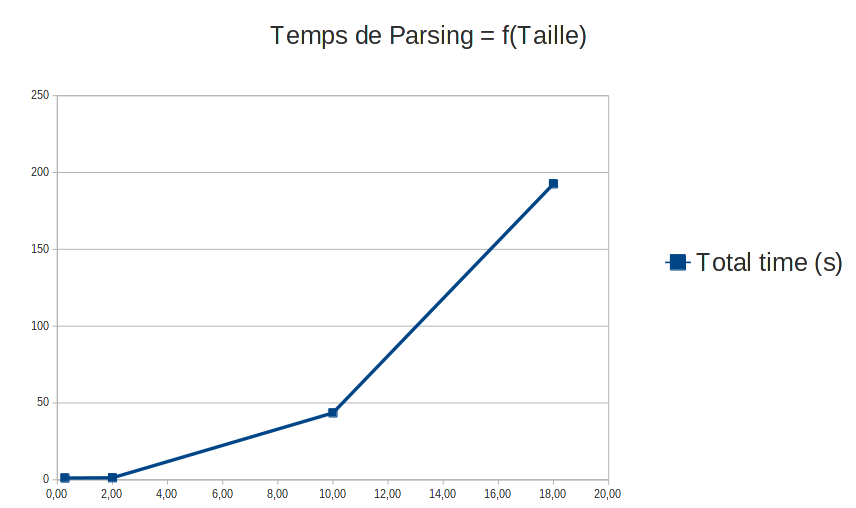
\includegraphics[scale=0.3]{parse-temps.png}
    \end{center} 
  \end{frame}

  
 \section{Démonstration}

  %Ici une démonstration live de 5 min

  \section{Travail à venir}
  \begin{frame}
    Scénario d'utilisation
    \begin{itemize}
     \item Upload du fichier Pcap, affichage en continu des données analysées
     \item Liste des protocoles / hosts avec des chiffres dans la sidebar
     \item Vue treemap qui permet de caractériser les hosts, filtrage dans la
     barre à gauche
     \item Passage en coordonées parallèle avec seulement les hôtes filtrés qui
     permet de valider les hypothèses
     \item Vue géographique ?
    \end{itemize}
  \end{frame}
  
  \begin{frame}
    Problématiques à venir
    \begin{itemize}
     \item Technos suffisantes ? Tests de performance à venir
     \item Morcellement de l'analyse du Pcap
     \item Création de vues interactives, et donc d'une belle architecture de
     données
     \end{itemize}
  \end{frame}
  
  \begin{frame}
    Objectifs à remplir
    \begin{itemize}
     \item Ajouter les différents filtres possibles
     \item Extraire d'un pcap a partir des trames filtrées
     \item Extraire les données non chiffrées des protocoles SMTP,IMAP,POP,LDAP
     \item Ajouter la résolution DNS
     \item Ajouter d'autres mode de visualisation (carte des IP,..)
    \end{itemize}
  \end{frame}


  \section{Conclusion}
  \begin{frame}
    \begin{center}
      Merci de votre attention ! \\
      https://github.com/lechinoix/Pcap-visualization-project
    \end{center}
  \end{frame}

\end{document}
